\documentclass[landscape]{infslides}
\usepackage{graphicx}
\usepackage{multicol}
\usepackage[export]{adjustbox}
\graphicspath{{./images/}}
\begin{document}

\title[IoTSSC Project]{IoTSSC Project\\Indoor Localisation}
\author[Lorenzo Martinico and Piotr Jander]{Lorenzo Martinico \and Piotr Jander}
\date{\today}

\maketitle
%\tableofcontents
\begin{slide}{Tracking device}
    Our chosen localisation device is a Nordic nRF51-DK, running ARM Mbed OS 5
    \begin{figure}
        \centering
        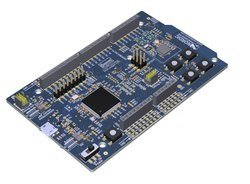
\includegraphics{nRF51-DK.jpg}
    \end{figure}
    Due to limited processing power, the firmware running on the board is limitied to scanning for Bluetooth Beacons and updating a BLE Characteristic with their RSSI strength
\end{slide}
\begin{slide}{Android App}
    \begin{multicols}{2}
        The app acts as a Bluetooth gateway, connecting to the board to read from its LocationService, and forward a timestamped RSSI, BeaconID pair to the server.\\
        Additionally, we display a map of the 5th floor, and a location marker, which can be manually modified based on the board's position to collect training data.
        \begin{figure}
            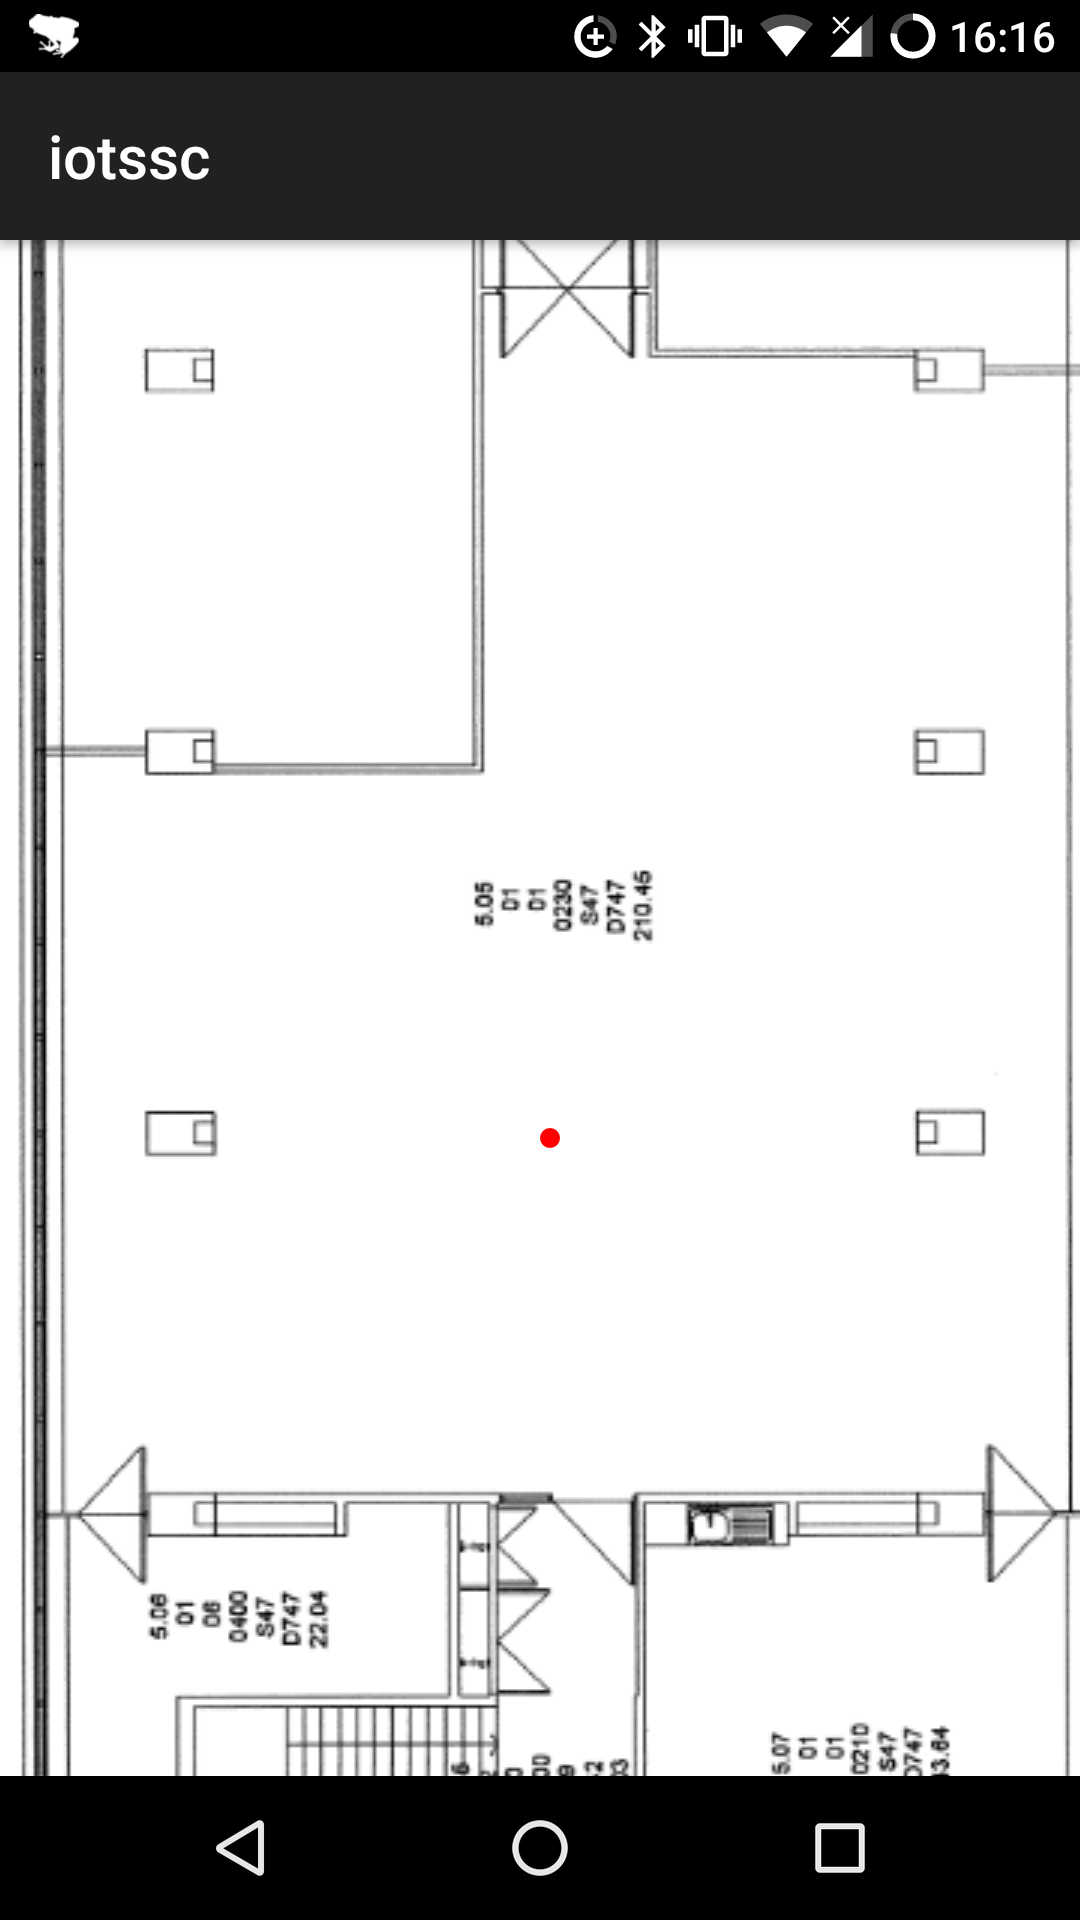
\includegraphics[scale=0.2,right]{Screenshot.png}
        \end{figure}
    \end{multicols}
\end{slide}
\begin{slide}{Server}
The server is a simple Flask app hosted on a Google Cloud Virtual Machine. It receives POST requests from the Gateway, and saves the data in a file.

To ensure all data is transimitted securely, the server runs over HTTPS, using a self signed certificate manually provisioned to the app (its only client).
\end{slide}
\begin{slide}{Analytics}
    ...
    RSSI triangulation 
    SVMs
    KNN
    Kalman Filters
\end{slide}
\end{document}

